\chapter{Implementation}


\section{Implementation Language Choice}

The compiler will be implemented using the Haskell programming language.

During complication the need to traverse trees usually occurs quite
often. Functional languages like Haskellare suited to this task 
due to features such as pattern matching and tail-end recursive optimisation 
which make traversing trees efficient and simple to implement/ 

The Glasgow Haskell Compiler is available for most platforms, most importantly for Windows, OSX and Linux 
on x86 architectures. This allows the compiler to be portable across these platforms provided the libraries 
used to build the compiler are portable.

Haskell has algebaric datatypes, these makes Abstract Syntax Trees
simpler to implement. For example the AST for a very simple expression
can be representedas follows:

\begin{lstlisting}[style=myHaskell]

    data Expression =
          Add Expression Expression
        | Negate Expression 
        | Const Integer

\end{lstlisting}

The equivalent in an Imperative/OOP language (in this case Java)
would be the following:

\begin{lstlisting}[style=myJava]

abstract Class Expression {}

class Add extends Expression {
    public Expression left;
    public Expression right;
    public Add(Expression l, Expression r) {
        left = l;
        right = r;    
    } 
}

class Negate extends Expression {
    public Expression expr;
    public Negate(Expression e) {
        expr = e;    
    }
} 

class Const extends Expression {
    public int value;
    public Const(int v) {
        value = v;
    }
}       

\end{lstlisting}

The Haskell version is much clearer on the structure of the tree, and takes much
less code to implement. 

It is also to easily extend Haskell datatypes to include
custom annotations. For example storing the source code position for parts of expressions may
be useful for reporting errors to the user.

Due to the pure function nature of Haskell, parts of complilation can easily be performed in parallel.
For example during type checking, each GPC function can be type checked in parallel and this can even be subdivided 
further into blocks within functions. For this project parallisation is not a concern, but in the future if compliation ever
needs to be faster then this option is always available.

Haskell also has powerful libraries for parsing source code such as Parsec which is a parser combinator
library. Parsec allows Combinator parsers to be written in the Haskell language itself avoiding the complexity
of integration of different tools and languages. 
\cite{parsec}

\section{Tools and Testing}

\subsection{Cabal}

Cabal (Common Architecture for Building Applications and Libraries) is a system for building and
packaging Haskell libraries and programs.\cite{cabal}. Using this system to manage the
project library dependencies, and can automatically download and install missing dependencies,
build and install the compiler on the system, and run unit tests simply.

\subsection{Testing}

For Unit testing the HUnit library will be used, this can be integrated
with Cabal to easily run unit tests.

One form of testing used for this project is testing each individual component.
(e.g. The Parser, The TypeChecker) Each component in the compiler can easily
be uncoupled from one another due to the linear nature of compliation.

Another form of testing is writing GPC source files which should compile, and
GPC files which should fail compilation at a certain stage, the compiler
is then invoked during testing on all of these files to check whether
all the source files which should compile do infact compile with no errors,
and all the source files which should raise an error do not compile.

An upside to this method is that testing this way is flexible in that
they aren't coupled with the implementation internals of the compiler.
The only way that these test would need to be changed was if the design
of the language itself would need to be changed.

The downsides to this method is that without manually checking the errors raised
by the tests that should fail the source may generate an error which is unrelated
to the error that is being tested. This is why some testing of each internal
component is done alongside this method.

\subsection{Code Coverage}

The Haskell HPC (Haskell Program Coverage) library allows for recording
code coverage over different modules during testing. This can be integrated with
cabal unit testing to automatically generate these results. The usefulness of this
allows for checking which sections of code still need to be tested and assists
in writing further unit tests.


\section{Structure}
Compilation is split up into multiple stages or "passes",
it is possible to compile in one pass but modularising each 
specific section of compilation allows modularity and decoupling.

This flow chart illustrates the basic structure of the Compiler
and its multiple stages:


\begin{center}
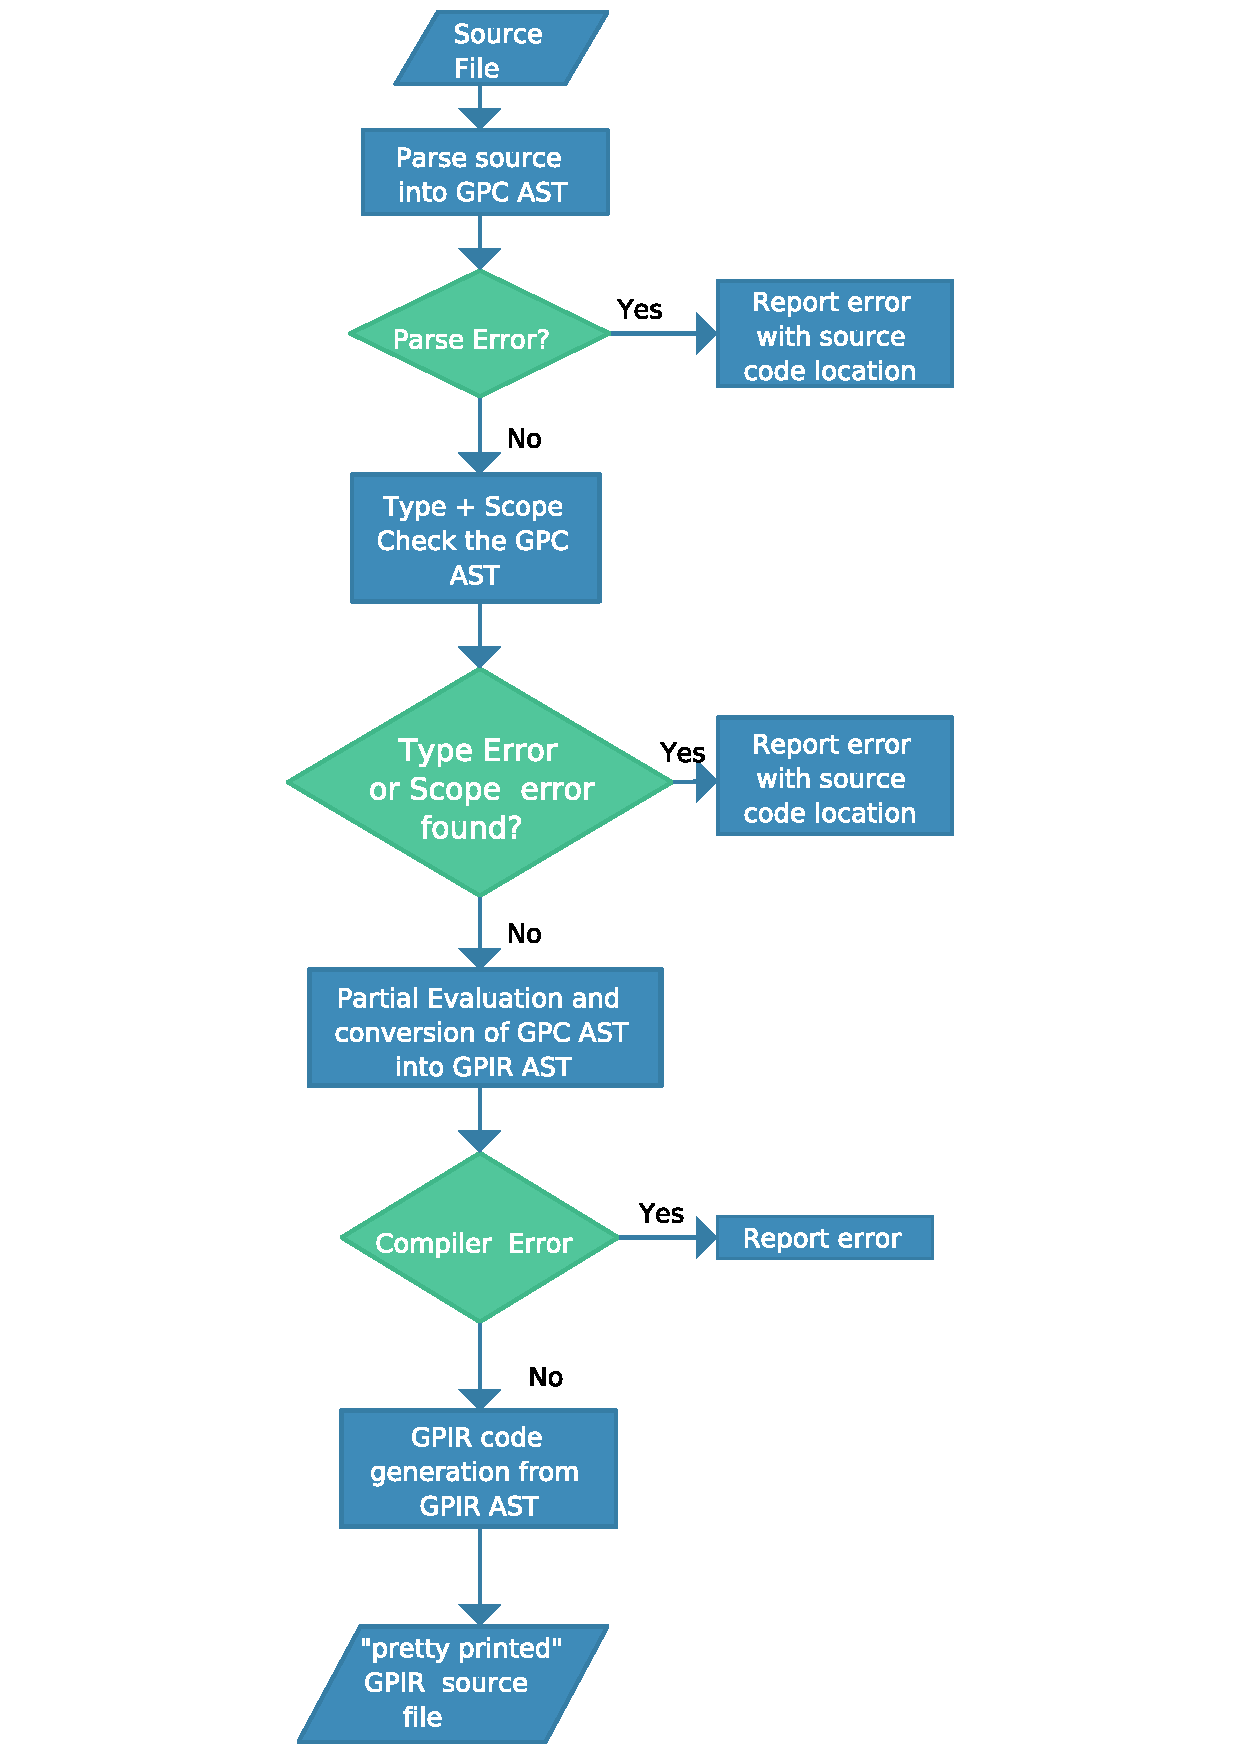
\includegraphics{graphs/Dissertation.pdf}
\end{center}
    
\subsection{Parser/Lexer}


\subsection{Type and Scope checking}

Type and Scope checking is done together as. to check the type of
an expression, the variables have to be in scope to get the type from.
The idea is to first type and scope check all top level constructs (object declarations, constuctors,
assignments) then map the checker over all functions.

For checking over top level statements we have a data structure as follows:

\begin{lstlisting}[style=myHaskell]
type VarTable = M.Map (Ident SrcPos) (Type SrcPos)
type FunTable = M.Map (Ident SrcPos) (Type SrcPos, [Type SrcPos])
type ObjectTable = M.Map (Ident SrcPos) (Objects SrcPos)

data MainBlock = MainBlock {
    _tlFuncDefs      :: FunTable, -- ^ Function Definitions
    _tlVarTypes      :: VarTable,  -- ^ Top Level Constant variable types
    _objects         :: ObjectTable  -- ^ Table of current Kernel objects declared 
} deriving (Show)
\end{lstlisting}

We need to check no duplicate functions exist, no duplicate top level variables,
and that constructor assignments to objects are correct. Once all top level statements have
been checked, all functions in scope stores, all top level variables stored, and all variables stored.
We can then type and scope check each individual function.

We need a slightly different stucture to type check functions.

At anytime we need to know what variables we currently have in scope, their types,
what functions are avilable to call, their argument types, and return types. What objects
are available to call methods on. Also the current function we 

We can store these in a structure:

\begin{lstlisting}[style=myHaskell]

data CodeBlock = CodeBlock {
    _currentFun :: Ident SrcPos, -- ^ Name of Function block is in
    _funcDefs   :: FunTable, -- ^ Function names and return/argument types
    _prevVars   :: VarTable, -- ^ Identifiers visible in current scope with types
    _curVars    :: VarTable  -- ^ Identifiers declared in current scope
} deriving (Show)


\end{lstlisting}

When a function is being type check we need to create a new CodeBlock instance
from a MainBlock instance. Store the details of the function that is being entered
in "currentFun", copy all functions we have in scope to "funcDefs", and set prevVars
to all the top level variables, with objects (stored as an object variable type).


Whenever we encounter a new scope (calling a function, or a seq/par block)
we create a new CodeBlock structure using the current structure, with a new set
of curVars, current curVars set to prevVars. If encountering a new function
we set the currentFun. funcDefs is copied, as currently the language doesn't support
nested functions.   

Using the State Monad we can create new CodeBlocks by appearing to update values.
We can calculate the current scope as curVars remove prevVars as any variables declared
in the current scope that are present in the previous scope the current scope variable is used.
If the variable is only in the previous scope then that one is used.

When type checking a function we type check every statement in the function,
for every statement, we type check the expressions within the statement.

We use a custom ErrorMonad which contains error messages for specific errors,
using a monad stack with the State Monad. When we check for an error and lift
it into the stack, if an error is raised then type checking stops.

\subsection{Evaluation}
\subsection{GPIR Code Generation}
